%%%%%%%%%%%%%%%%%%%%%%%%%%%%%%%%%%%%%%%%%
% Beamer Presentation
% LaTeX Template
% Version 1.0 (10/11/12)
%
% This template has been downloaded from:
% http://www.LaTeXTemplates.com
%
% License:
% CC BY-NC-SA 3.0 (http://creativecommons.org/licenses/by-nc-sa/3.0/)
%
%%%%%%%%%%%%%%%%%%%%%%%%%%%%%%%%%%%%%%%%%

%------------------------------------------------------------------------------------------------
%	PACKAGES AND THEMES
%------------------------------------------------------------------------------------------------

\documentclass[table, xcolor = {dvipsnames}, 9pt]{beamer}
%\usepackage{beamerarticle}
\usepackage{tikz}
\usetikzlibrary{calc}
\usetikzlibrary{positioning}
\usetikzlibrary{arrows.meta}
\usetikzlibrary{external}
\mode<presentation> {

% The Beamer class comes with a number of default slide themes
% which change the colors and layouts of slides. Below this is a list
% of all the themes, uncomment each in turn to see what they look like.

\usetheme{default}
%\usetheme{AnnArbor}
%\usetheme{Antibes}
%\usetheme{Bergen}
%\usetheme{Berkeley}
%\usetheme{Berlin}
%\usetheme{Boadilla}
%\usetheme{CambridgeUS}
%\usetheme{Copenhagen}
%\usetheme{Darmstadt}
%\usetheme{Dresden}
%\usetheme{Frankfurt}
%\usetheme{Goettingen}
%\usetheme{Hannover}
%\usetheme{Ilmenau}
%\usetheme{JuanLesPins}
%\usetheme{Luebeck}
%\usetheme{Madrid}
\usetheme{metropolis}
%\usetheme{Malmoe}
%\usetheme{Marburg}
%\usetheme{Montpellier}
%\usetheme{PaloAlto}
%\usetheme{Pittsburgh}
%\usetheme{Rochester}
%\usetheme{Singapore}
%\usetheme{Szeged}
%\usetheme{Warsaw}

% As well as themes, the Beamer class has a number of color themes
% for any slide theme. Uncomment each of these in turn to see how it
% changes the colors of your current slide theme.

%\usecolortheme{albatross}
%\usecolortheme{beaver}
%\usecolortheme{beetle}
%\usecolortheme{crane}
%\usecolortheme{dolphin}
%\usecolortheme{dove}
%\usecolortheme{fly}
%\usecolortheme{lily}
%\usecolortheme{orchid}
%\usecolortheme{rose}
\usecolortheme{seagull}
%\usecolortheme{seahorse}
%\usecolortheme{whale}
%\usecolortheme{wolverine}
\usefonttheme{professionalfonts}
%\setbeamertemplate{footline} % To remove the footer line in all slides uncomment this line
%\setbeamertemplate{footline}[page number] % To replace the footer line in all slides with a simple slide count uncomment this line

%\setbeamertemplate{navigation symbols}{} % To remove the navigation symbols from the bottom of all slides uncomment this line
}

\usepackage{graphicx} % Allows including images
\usepackage{booktabs} % Allows the use of \toprule, \midrule and \bottomrule in tables
\usepackage{tikz}
\usepackage{multirow}
\usepackage{natbib}
\usepackage{hyperref}
\usepackage{diagbox}
\usepackage{makecell}
\usepackage{xparse}
\usepackage{subfig}
\usepackage{amsmath}
\usepackage{amsfonts,amsthm,amsmath,amssymb}
\usepackage{centernot}
\usepackage{bbm}
\usepackage{bm}
\usepackage{empheq}
\usepackage{pgfplots}
\usepackage{animate}
\usepackage[font = small, skip = 0pt]{caption}
\usepgfplotslibrary{colorbrewer}

\newcommand\mybox[2][]{\tikz[overlay]\node[fill=lightgray,inner sep=2pt, anchor=text, rectangle, rounded corners=1mm,#1] {#2};\phantom{#2}}
\hypersetup{unicode=true,
            bookmarksnumbered=true,
            bookmarksopen=true,
            bookmarksopenlevel=2,
            breaklinks=false,
            pdfborder={0 0 1},
            hypertexnames=false,
            pdfstartview={XYZ null null 1}}
\usepackage{xcolor}
\newcommand\myheading[1]{%
  \par\Bigskip
  {\Large\bfseries#1}\par\smallskip}
\newcommand\given[1][]{\:#1\vert\:}

\newcommand\MyBox[1]{%
    \fbox{\parbox[c][3cm][c]{3cm}{\centering #1}}%
    % Size of boxes
}
\newcommand\MyVBox[1]{%
    \parbox[c][1cm][c]{1cm}{\centering\bfseries #1}%
}
\newcommand\MyHBox[2][\dimexpr3cm+2\fboxsep\relax]{%
    \parbox[c][1cm][c]{#1}{\centering\bfseries #2}%
}
\newcommand\MyTBox[4]{%
    \MyVBox{#1}
    \MyBox{#2}\hspace*{-\fboxrule}%
    \MyBox{#3}\par\vspace{-\fboxrule}%
}
%%%%
\newcommand*\rot{\rotatebox{90}}
\theoremstyle{plain}
\newtheorem{thm}{Theorem}
\newtheorem{prop}{Proposition\thisthmnumber}
\newtheorem{lem}{Lemma\thisthmnumber}
\newtheorem{cor}{Corollary}
\newtheorem{defin}{Definition}
\newtheorem{algo}{Algorithm}
\newcommand*\diff{\mathop{}\!\mathrm{d}}
\newcommand*\Diff[1]{\mathop{}\!\mathrm{d^#1}}
\newcommand{\thisthmnumber}{}
\newcommand{\tikzmark}[1]{\tikz[baseline,remember picture] \coordinate (#1) {};}
\newcommand*{\QEDA}{\hfill\ensuremath{\blacksquare}}%
\newcommand*{\QEDB}{\hfill\ensuremath{\square}}%
\newcommand{\notimplies}{%
  \mathrel{{\ooalign{\hidewidth$\not\phantom{=}$\hidewidth\cr$\implies$}}}}
\DeclareMathOperator{\E}{\rm{E}}
\DeclareMathOperator{\R}{\mathbb{R}}
\DeclareMathOperator{\Var}{\rm{Var}}
\DeclareMathOperator{\Cov}{\rm{Cov}}
\DeclareMathOperator{\e}{\rm{e}}
\DeclareMathOperator{\logit}{\rm{logit}}
\DeclareMathOperator{\indep}{{\perp\!\!\!\perp}}
\DeclareMathOperator{\rank}{rank}
\DeclareMathOperator*{\argmin}{arg\,min}
\DeclareMathOperator*{\argmax}{arg\,max}
%\DeclareMathOperator{\Pr}{\rm{Pr}}
%------------------------------------------------------------------------
%	TITLE PAGE
%-----------------------------------------------------------------------
\pagestyle{empty}
\title[]{Causal Inference for the Social Sciences I} % The short title appears at the bottom of every slide, the full title is only on the title page

\author{Jake Bowers and Ben B. Hansen}
\institute[]
{

}
\date{}

\NewDocumentEnvironment{statement}{mo}
 {%
  \IfValueT{#2}{\renewcommand{\thisthmnumber}{ #2}}\begin{#1}%
 }
 {\end{#1}}

\begin{document}

\begin{frame}
\titlepage % Print the title page as the first slide
\end{frame}

%\begin{frame}
%\frametitle{Overview} % Table of contents slide, comment this block out to remove it
%\tableofcontents % Throughout your presentation, if you choose to use \section{} and \subsection{} commands, these will automatically be printed on this slide as an overview of your presentation
%\end{frame}

%------------------------------------------------------------------------
%	PRESENTATION SLIDES
%-------------------------------------------------------------------------------------
\section{Instructional Team}
\begin{frame}[t]
\frametitle{Instructor}
\vfill
\href{https://dept.stat.lsa.umich.edu/~bbh/}{Ben B. Hansen}
\begin{itemize} \vfill
\item Professor, Statistics Department, University of Michigan
\end{itemize} \vfill
\begin{figure}[H]
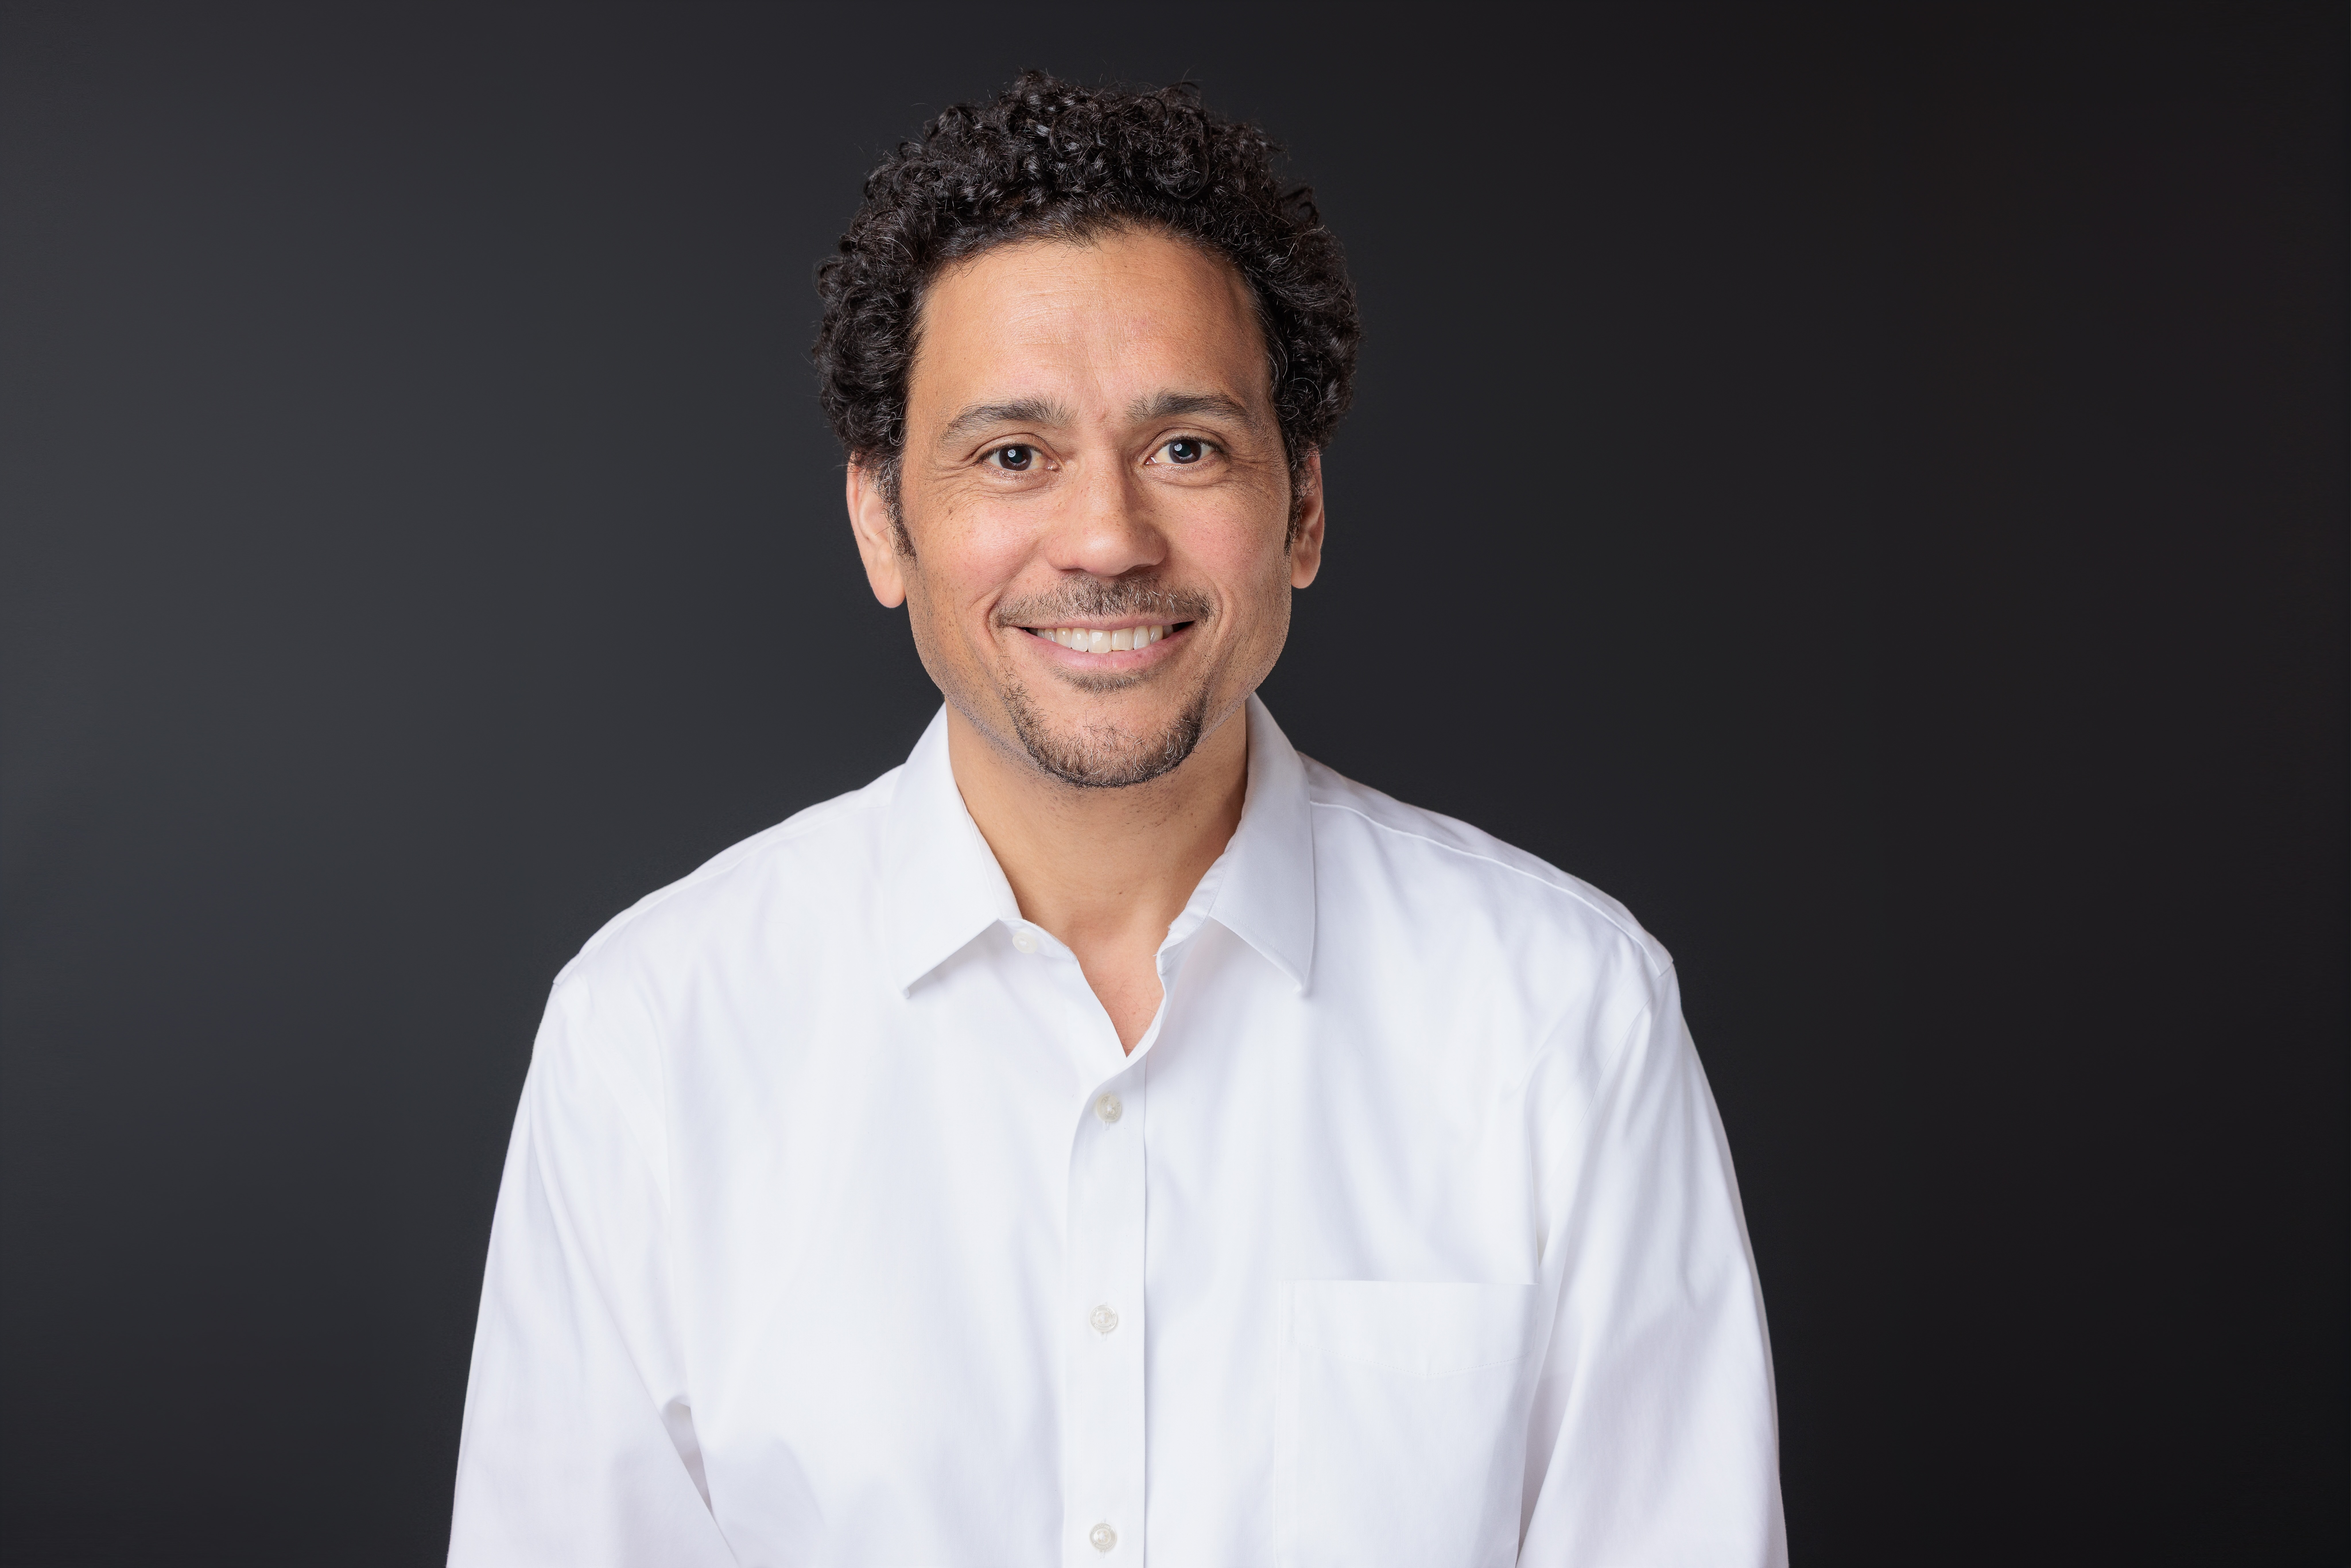
\includegraphics[width=0.75\linewidth]{bbhansen_photo_2025_3x2_f-smile_hi-res.jpg}%
\end{figure}
\vfill
\end{frame}
%-------------------------------------------------------------------------------------
\begin{frame}[t]
\frametitle{Instructor}
\vfill
\href{https://www.jakebowers.org/}{Jake Bowers}
\begin{itemize} \vfill
\item Professor, Departments of Political Science \&  Statistics,
  University of Illinois @ Urbana-Champaign (UIUC)
\end{itemize} \vfill
\begin{figure}[H]
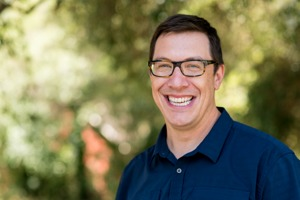
\includegraphics[width=0.75\linewidth]{jakeBowers.jpg}%
\end{figure}
\vfill
\end{frame}
%-------------------------------------------------------------------------------------
\begin{frame}[t]
\frametitle{Teaching Assistants (TAs)}
\vfill
\href{https://www.alicemalmberg.com/}{Alice Malmberg} \vfill
\begin{itemize} \vfill
\item Ph.D.~Candidate, Political Science, University of California, Davis \vfill
\end{itemize} \vfill
\href{https://pol.illinois.edu/directory/profile/ak72}{Abdullah Kabaoglu} \vfill
\begin{itemize} \vfill
\item Ph.D.~Student, Political Science, University of Illinois
\end{itemize} \vfill
\vfill
\end{frame}
%-------------------------------------------------------------------------------------
\section{Course outline}
\begin{frame}[t]
\frametitle{Course outline}
\vfill
\begin{enumerate} \vfill
\item[] We cover methods including  \vfill
  \begin{itemize}\vfill
    \item Randomization-based analysis for experiments, in Fisher's or
      Neyman's style\vfill
  \item Instrumental variables \& principal stratification  \vfill
  \item Propensity scores and matching  \vfill
  \item Omitted variable sensitivity analysis  \vfill
  \end{itemize}\vfill 
\item[] \textcolor{magenta}{Part 1: The randomized experimental ideal} \vfill
\begin{itemize} \vfill
\item Introduction to potential outcomes and random assignment \vfill
\item Estimation and inference in fully controlled randomized experiments \vfill
\end{itemize} \vfill
\item[] \textcolor{magenta}{Part 2: Imperfectly controlled randomized experiments} \vfill
\begin{itemize} \vfill
\item Noncompliance: When subjects don't comply with experiment's treatment \vfill
\item Attrition: When subjects don't report their outcomes \vfill
\end{itemize} \vfill
\item[] \textcolor{magenta}{Part 3: Observational studies (when subjects self-select into treatment)} \vfill
\begin{itemize} \vfill
\item Matching and assessments of ``covariate balance'' \vfill
\item Depending on interest, other designs we may cover include regression discontinuity, difference-in-differences, interrupted time series, synthetic control, etc. \vfill
\end{itemize} \vfill
\item[] \textcolor{magenta}{Part 4: Sensitivity analysis} \vfill
\begin{itemize} \vfill
\item How would inferences change should crucial assumptions be false? \vfill
\end{itemize} \vfill
\end{enumerate}
\vfill
\end{frame}
%-------------------------------------------------------------------------------------
\begin{frame}[t]
\frametitle{Course outline}
\vfill
\begin{itemize} \vfill
\item Part 1 of the course is very conceptual, covering essential topics in statistics but from a new \textcolor{magenta}{randomization- or design-based} perspective \vfill
\begin{itemize} \vfill
\item[$\star$] This part of the course is often the most challenging \vfill
\end{itemize} \vfill
\item Parts 2 - 4 emphasize computation in \texttt{R} \vfill
\begin{itemize} \vfill
\item Especially \texttt{R}'s \texttt{optmatch} package \vfill
\end{itemize} \vfill
\end{itemize} \vfill
\vfill
\end{frame}
%-------------------------------------------------------------------------------------
\section{Objectives, Audience, Prerequisites \& Materials}
\begin{frame}[t]
\frametitle{Audience and Prerequisites}
\vfill
\begin{itemize} \vfill
\item The typical student is an applied scientist who plans to use causal inference in their research \vfill
\item Exposure to \texttt{R} is helpful, but not necessary \vfill
\item Familiarity with statistical concepts is assumed: random variables, expectations, distribution functions, etc ...
\begin{itemize} \vfill
\item Familiarity with regression, maximum likelihood, etc is less important \vfill
\end{itemize}  \vfill 
\end{itemize} \vfill
\vfill
\end{frame}
%-------------------------------------------------------------------------------------
\begin{frame}[t]
\frametitle{Learning objectives}
\vfill
Students will learn to:
\begin{enumerate} \vfill
\item Distinguish, apply and evaluate needs for causal inference
  assumptions flowing research design.  \vfill
\item Perform randomization inferences for randomized trials in R,
  including those with clustered or stratified treatment allocation
  and/or imperfect compliance. Appropriately adapt these inference
  strategies to observational studies, and to diagnostics including
  covariate balance.\vfill
\item Perform or critique statistical adjustments for
  observational studies with the linear model and/or matching.\vfill
 \item Implement testing, estimation, and adjustment methods covered in the course using R, in replicable scripts combining R and markdown.
\end{enumerate} \vfill
\vfill
\end{frame}
%-------------------------------------------------------------------------------------
\begin{frame}[t]
\frametitle{Textbooks and assignments}
\vfill
\begin{itemize} \vfill
\item Primary textbook: \citet{rosenbaum2017} \vfill
\begin{itemize}
\item Supplementary textbooks: \citet{rosenbaum2002,rosenbaum2010,imbensrubin2015,gerbergreen2012} \vfill
\end{itemize}    
\item Three homework assignments \vfill
\begin{itemize} \vfill
\item Mix of conceptual questions and applied questions with data analysis using \texttt{R} \vfill
\end{itemize} \vfill
\end{itemize} \vfill
\vfill
\begin{block}{}
{\scriptsize
\bibliographystyle{chicago}
\bibliography{bibliography}   % name your BibTeX data base
}
  \end{block}
\end{frame}
%-------------------------------------------------------------------------------------
%---------------------------------------------------------------
\end{document}